\documentclass%[handout]%
{beamer}
%\usetheme{Execushares}
%\usetheme{AnnArbor}
\usetheme{Copenhagen}
\usecolortheme{beaver}
%\setbeamercolor{title}{parent=structure,bg=green!50!black,fg=white}
%\usecolortheme{dolphin}
\setbeamertemplate{navigation symbols}{}%remove navigation symbols

\usepackage{amsmath}
\usepackage{amssymb}
\usepackage{amsthm}
%\usepackage[utf8]{inputenc}
\usepackage[czech]{babel}
\usepackage{tikz-cd}
\usepackage[mathscr]{euscript}
\usepackage[IL2]{fontenc}
\usepackage{mathtools}

\usetikzlibrary{calc,shapes.callouts,shapes.arrows,shapes.symbols}

%\usepackage{beamerarticle}

%\usepackage{bbm}

\def\rllap#1{\hbox to0pt{\hss#1\hss}}

%\newcommand{\bubblethis}[2]{
        %\tikz[remember picture,baseline]{\node[anchor=base,inner sep=0,outer sep=0]%
        %(#1) {\underline{#1}};\node[overlay,cloud callout,callout relative pointer={(-0.2cm,+0.7cm)},%
        %aspect=2.5,fill=yellow!90] at ($(#1.north)+(-0.5cm,1.6cm)$) {#2};}%
    %}%
		%
%\newcommand{\speechthis}[2]{
        %\tikz[remember picture,baseline]{\node[anchor=base,inner sep=0,outer sep=0]%
        %(pom) {#1};\node[overlay,ellipse callout,fill=blue!50] 
        %at ($(pom.north)+(1cm,+0.8cm)$) {#2};}%
    %}%
		%

\newcommand{\DO}{\mathrm{D}}
\newcommand{\HO}{\mathrm{H}}

\title{Funkce}
\author{Alexander Slávik} %  and J. Trlifaj
\subtitle{Úvod}
\institute{Gymnázium Voděradská}
% \date{5. 10. 2020}
\date{4. 10. 2022}

\begin{document}


\frame{\titlepage}


\section{Základy}

\begin{frame}
	\frametitle{Definice}
	
	\pause
	Matematika pro gymnázia -- Funkce (Doc.\ RNDr.\ Oldřich Odvárko, DrSc.):
	
	\pause
	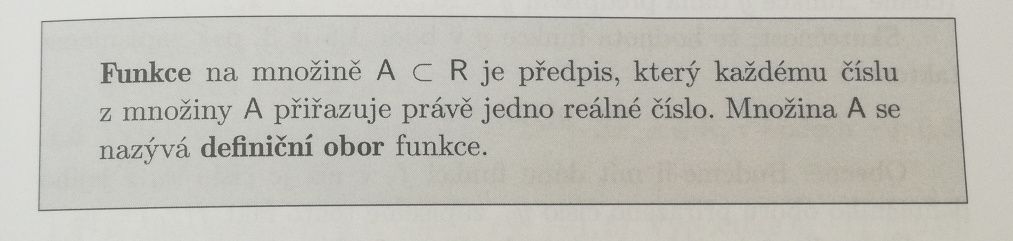
\includegraphics[width=\hsize]{def_fce.jpg}
	
	\bigskip\bigskip
	
	\pause
	\uv{Lepší} definice bude v semináři z difernciálního a integrálního počtu.
\end{frame}


\begin{frame}
	\frametitle{Jiná představa}
	
	\[ \begin{tikzpicture}
		\fill[black] (-1,-1) rectangle (1,1);
		\node[white] at (0,0) {\LARGE $f$};
		\begin{scope}[thick]
				\draw (-3,2) -- (-1,1);
				\draw (-3,-2) -- (-1,-1);
				\draw (3,2) -- (1,1);
				\draw (3,-2) -- (1,-1);
		\end{scope}
		\pause
		\node[red] at (-3,0) {$x$};
		\draw[->] (-2.5,0) -- (-1.5,0);
		\pause
		\node[blue] at (3,0) {$f(x)$};
		\draw[->] (1.5,0) --  (2.5,0);
		\onslide<1->
	\end{tikzpicture}	\]
	
\end{frame}


\begin{frame}
	\frametitle{Identická funkce}
	
	\[ \begin{tikzpicture}
		\fill[black] (-1,-1) rectangle (1,1);
		\node[white] at (0,0) {\LARGE $f$};
		\begin{scope}[thick]
				\draw (-3,2) -- (-1,1);
				\draw (-3,-2) -- (-1,-1);
				\draw (3,2) -- (1,1);
				\draw (3,-2) -- (1,-1);
		\end{scope}
		\pause
		
		\begin{scope}[shift={(0,.5)}]
		\node[red] at (-3,0) {$1$};
		\draw[->] (-2.5,0) -- (-1.5,0);
		\end{scope}
		\pause
		\begin{scope}[shift={(0,.5)}]
		\node[blue] at (3,0) {$1$};
		\draw[->] (1.5,0) --  (2.5,0);
		\end{scope}
		
		\pause
		%\begin{scope}%[yshift=.5]
		\node[red] at (-3,0) {$6$};
		\draw[->] (-2.5,0) -- (-1.5,0);
		%\end{scope}
		\pause
		\node[blue] at (3,0) {$6$};
		\draw[->] (1.5,0) --  (2.5,0);
		%\end{scope}
		
		\pause
		\begin{scope}[shift={(0,-.5)}]
		\node[red] at (-3,0) {$\sqrt3$};
		\draw[->] (-2.5,0) -- (-1.5,0);
		\end{scope}
		\pause
		\begin{scope}[shift={(0,-.5)}]
		\node[blue] at (3,0) {$\sqrt3$};
		\draw[->] (1.5,0) --  (2.5,0);
		\end{scope}
		
		
		\onslide<1->
	\end{tikzpicture}	\]
	
	\pause
	
	\begin{center}
	\uv{Dostaň $x$, vrať $x$.}
	\end{center}
	
\end{frame}



\begin{frame}
	\frametitle{Kvadratická funkce \uv{$x^2$}}
	
	\[ \begin{tikzpicture}
		\fill[black] (-1,-1) rectangle (1,1);
		\node[white] at (0,0) {\LARGE $f$};
		\begin{scope}[thick]
				\draw (-3,2) -- (-1,1);
				\draw (-3,-2) -- (-1,-1);
				\draw (3,2) -- (1,1);
				\draw (3,-2) -- (1,-1);
		\end{scope}
		\pause
		
		\begin{scope}[shift={(0,.5)}]
		\node[red] at (-3,0) {$1$};
		\draw[->] (-2.5,0) -- (-1.5,0);
		\end{scope}
		\pause
		\begin{scope}[shift={(0,.5)}]
		\node[blue] at (3,0) {$1$};
		\draw[->] (1.5,0) --  (2.5,0);
		\end{scope}
		
		\pause
		%\begin{scope}%[yshift=.5]
		\node[red] at (-3,0) {$6$};
		\draw[->] (-2.5,0) -- (-1.5,0);
		%\end{scope}
		\pause
		\node[blue] at (3,0) {$36$};
		\draw[->] (1.5,0) --  (2.5,0);
		%\end{scope}
		
		\pause
		\begin{scope}[shift={(0,-.5)}]
		\node[red] at (-3,0) {$\sqrt3$};
		\draw[->] (-2.5,0) -- (-1.5,0);
		\end{scope}
		\pause
		\begin{scope}[shift={(0,-.5)}]
		\node[blue] at (3,0) {$3$};
		\draw[->] (1.5,0) --  (2.5,0);
		\end{scope}
		
		
		\onslide<1->
	\end{tikzpicture}	\]
	
	\pause
	
	\begin{center}
	\uv{Dostaň $x$, vrať druhou mocninu $x$.}
	\end{center}
	
	
\end{frame}




\begin{frame}
	\frametitle{Ještě jiný příklad}
	
	\[ \begin{tikzpicture}
		\fill[black] (-1,-1) rectangle (1,1);
		\node[white] at (0,0) {\LARGE $f$};
		\begin{scope}[thick]
				\draw (-3,2) -- (-1,1);
				\draw (-3,-2) -- (-1,-1);
				\draw (3,2) -- (1,1);
				\draw (3,-2) -- (1,-1);
		\end{scope}
		\pause
		
		\begin{scope}[shift={(0,.5)}]
		\node[red] at (-3,0) {$1$};
		\draw[->] (-2.5,0) -- (-1.5,0);
		\end{scope}
		\pause
		\begin{scope}[shift={(0,.5)}]
		\node[blue] at (3,0) {$1$};
		\draw[->] (1.5,0) --  (2.5,0);
		\end{scope}
		
		\pause
		%\begin{scope}%[yshift=.5]
		\node[red] at (-3,0) {$6$};
		\draw[->] (-2.5,0) -- (-1.5,0);
		%\end{scope}
		\pause
		\node[blue] at (3,0) {$4$};
		\draw[->] (1.5,0) --  (2.5,0);
		%\end{scope}
		
		\pause
		\begin{scope}[shift={(0,-.5)}]
		\node[red] at (-3,0) {$\sqrt3$};
		\draw[->] (-2.5,0) -- (-1.5,0);
		\end{scope}
		\pause
		%\begin{scope}[shift={(0,-.5)}]
		%\node[blue] at (3,0) {$3$};
		%\draw[->] (1.5,0) --  (2.5,0);
		%\end{scope}
		
		\node[starburst, draw, minimum width=3cm, minimum height=2cm,red,fill=yellow!50!orange,line width=1.5pt] at (2,-.5) {$\sqrt3 \notin \DO_f$};
		
		\onslide<1->
	\end{tikzpicture}	\]
	
	\pause
	
	\begin{center}
	\uv{Dostaň $x$, vrať počet (kladných) dělitelů čísla $x$.}
	\end{center}
	
	\pause
	
	%\medskip
	
	\begin{center}
	funkce $\approx$ předpis $\approx$ přiřazení $\approx$ proces
	\end{center}
	
	
\end{frame}



\begin{frame}
	\frametitle{Definiční obor \& obor hodnot}
	
	
	\begin{block}{Definiční obor}\pause
	\dots\ funkce $f$ značíme $\DO_f$ (příp. $\DO(f)$);
	
	\medskip\pause
	
	= množina těch reálných čísel $x$, pro která je hodnota $f(x)$ definována.
	
	\medskip\pause
	= \uv{co můžeme do $f$ dosadit}.
	\end{block}
	
	
	\pause
	\begin{block}{Obor hodnot}\pause
	\dots\ funkce $f$ značíme $\HO_f$ (příp. $\HO(f)$);
	
	\medskip\pause
	
	= množina těch reálných čísel $y$, pro která existuje aspoň jedno $x \in \DO_f$ splňující $y = f(x)$.
	
	\medskip\pause
	
	= \uv{jakých hodnot může $f$ nabývat}.
	\end{block}
	
	
	
\end{frame}



%\end{document}


\section{Zadání funkce}


\begin{frame}
	\frametitle{Jak funkci \uv{zadat}?}
	SŠ učebnice typicky uvádí tyto způsoby:\pause
	\begin{itemize}
		\item tabulkou,\pause
		\item grafem,\pause
		\item funkčním předpisem.%\pause
	\end{itemize}
\end{frame}


\begin{frame}
	\frametitle{Funkce daná tabulkou}
	Např. počet pozitivních testů na COVID-19 v ČR v $x$-tý den počínaje 1.~3.~2020:
	\pause
	\[
	\tiny
	%\tabskip=1pt
	\setlength{\tabcolsep}{1.2pt}
	\begin{tabular}{c*{33}{|c}}
	%1 & 2 & 3 & 4 & 5 & 6 & 
	den&
	1&2&3&4&5&6&7&8&9&10&11&12&13&14&15&16&17&18&19&20&21&22&23&24&25&26&27&28&29&30&31&32&\dots\\ \hline
	počet&
3&0&2&1&3&11&7&6&6&25&31&22&25&48&109&85&67&110&206&124&159&115&126&185&292&259&377&263&159&184&304&283&\dots
	\end{tabular}
	\]
	
	\medskip\pause
	Zřejmě může mít pouze konečný definiční obor a obor hodnot.
\end{frame}

\begin{frame}
	\frametitle{Funkce daná grafem}
		
	\[ 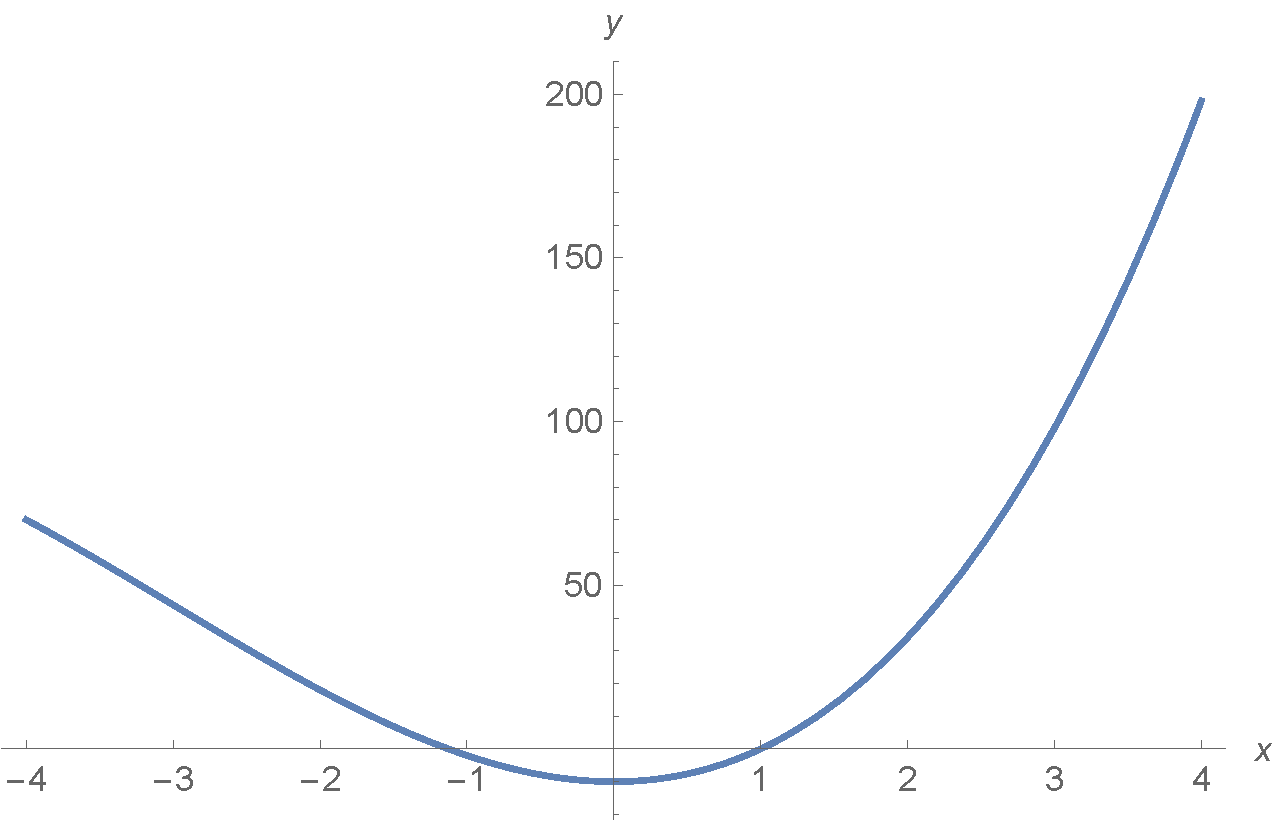
\includegraphics[height=.6\vsize]{cubic.pdf} \]
	
	\pause
	Takto \uv{zadaná} funkce musí mít \emph{omezený} definiční obor.
	
\end{frame}


\begin{frame}
	\frametitle{Funkce daná grafem II}
		
	\[ 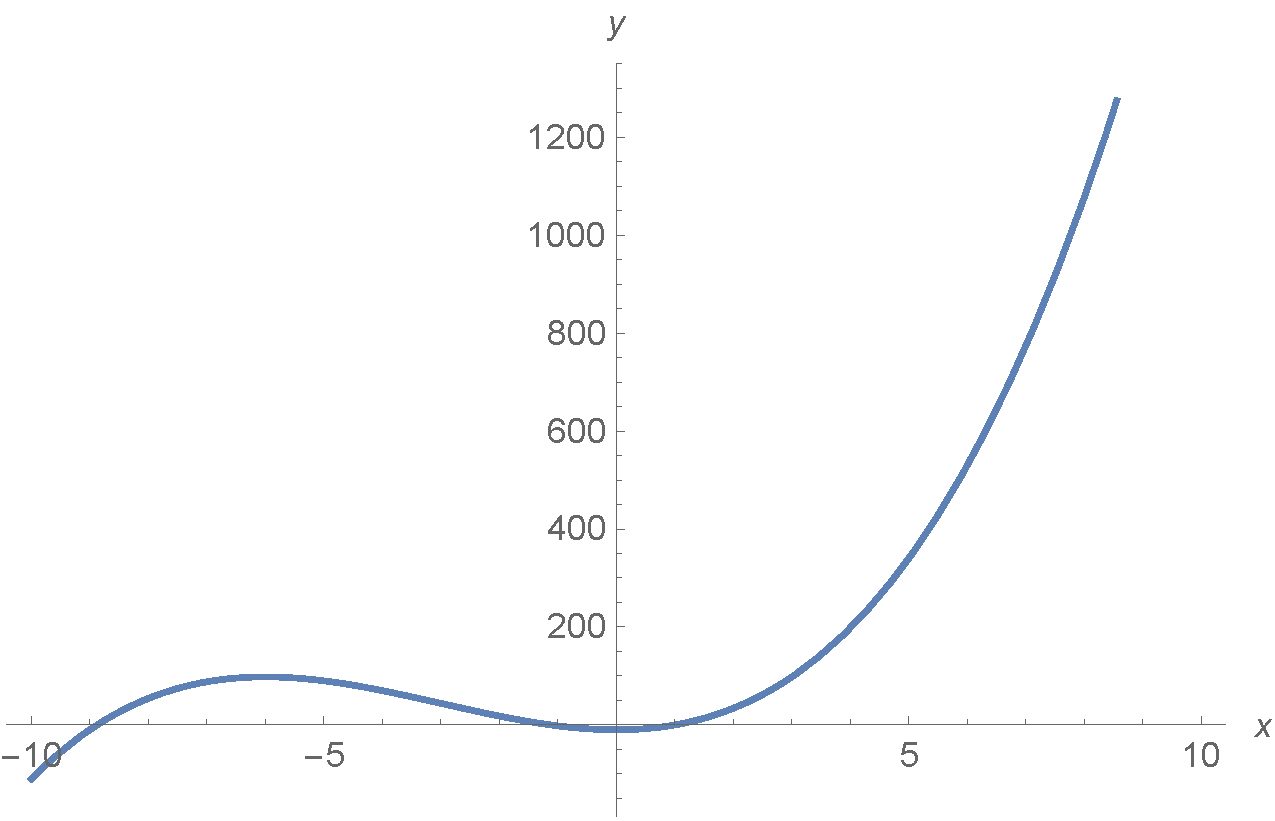
\includegraphics[height=.6\vsize]{cubic2.pdf} \]
	
	\pause
	Nezbytně záleží na tom, \uv{kam se díváme}. \pause ($y = x^3 + 9x^2 - 10$)
	
\end{frame}

\begin{frame}
	\frametitle{Funkce daná grafem III}
		
	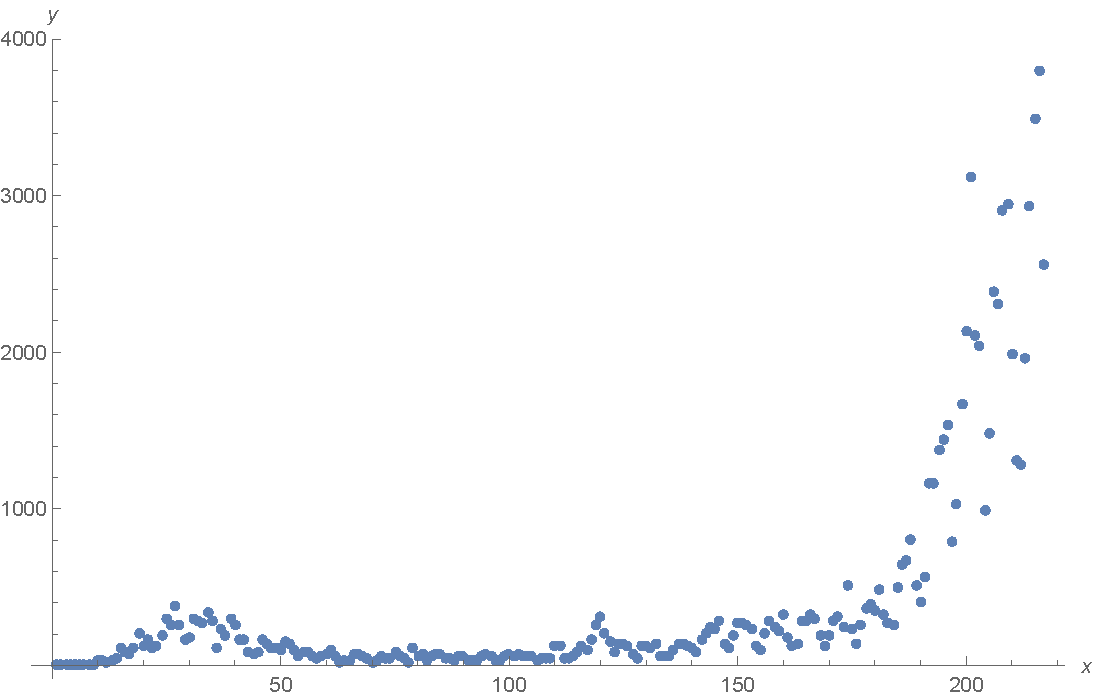
\includegraphics[height=.8\vsize]{covid.pdf}
	
	%\pause
	%Nezbytně záleží na tom, \uv{kam se díváme}. \pause ($y = x^3 + 9x^2 - 10$)
	
\end{frame}


\begin{frame}
	\frametitle{Funkce daná grafem III}
		
	Ze stránek Ministerstva zdravotnictví:
	
	\smallskip
	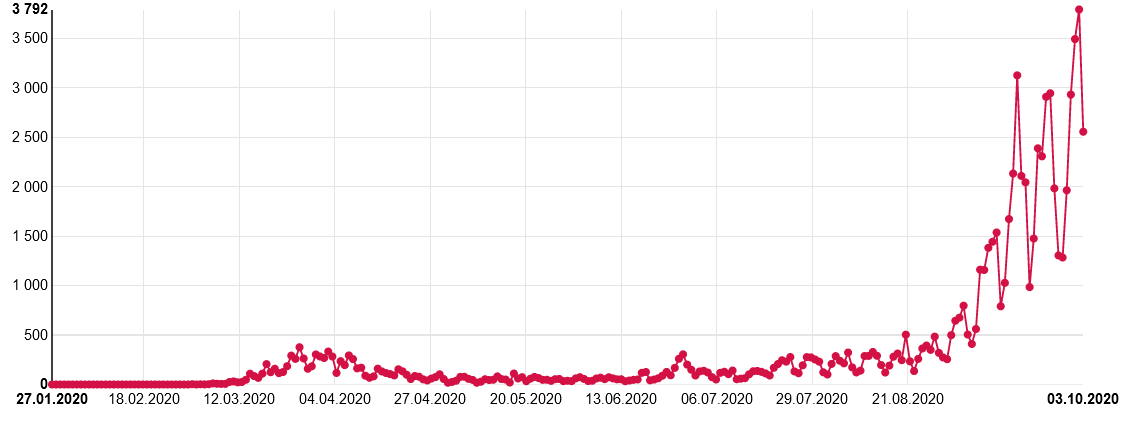
\includegraphics[width=\hsize]{covid_mz.png}
	
	\medskip\pause
	\uv{Spojování bodů} je přehledné, ale nemá matematický význam.
	%\pause
	%Nezbytně záleží na tom, \uv{kam se díváme}. \pause ($y = x^3 + 9x^2 - 10$)
	
\end{frame}


\begin{frame}
	\frametitle{Funkce daná grafem IV}
		
	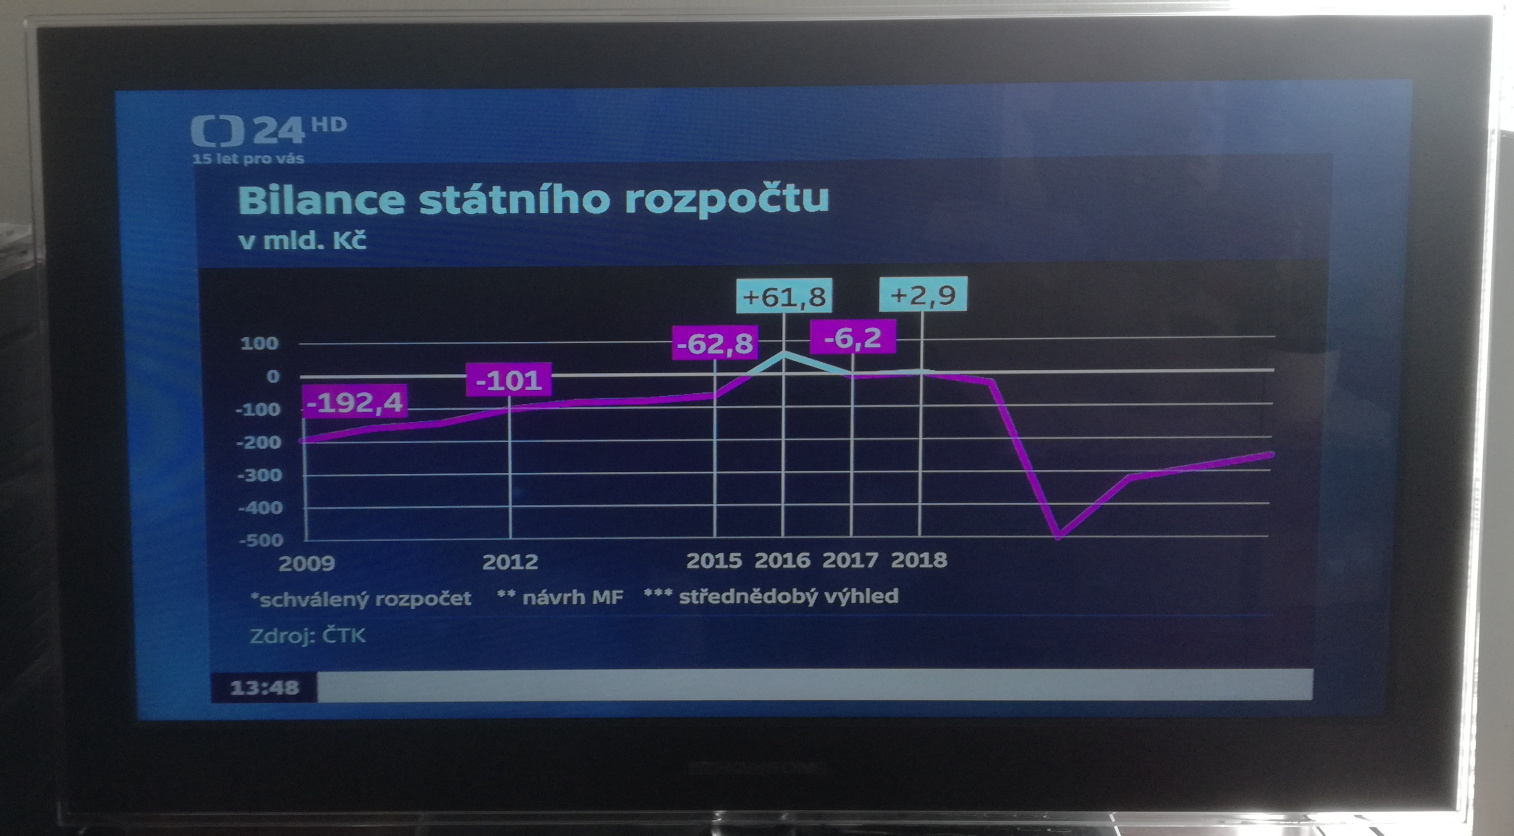
\includegraphics[width=\hsize]{tv.jpg}
	
	%\medskip\pause
	%\uv{Spojování bodů} je přehledné, ale nemá matematický význam.
	%\pause
	%Nezbytně záleží na tom, \uv{kam se díváme}. \pause ($y = x^3 + 9x^2 - 10$)
	
\end{frame}


\begin{frame}
	\frametitle{Funkce daná grafem V}
	
	Noty jakožto graf funkce:\pause\par\smallskip
		
	\hbox to\hsize{\hfil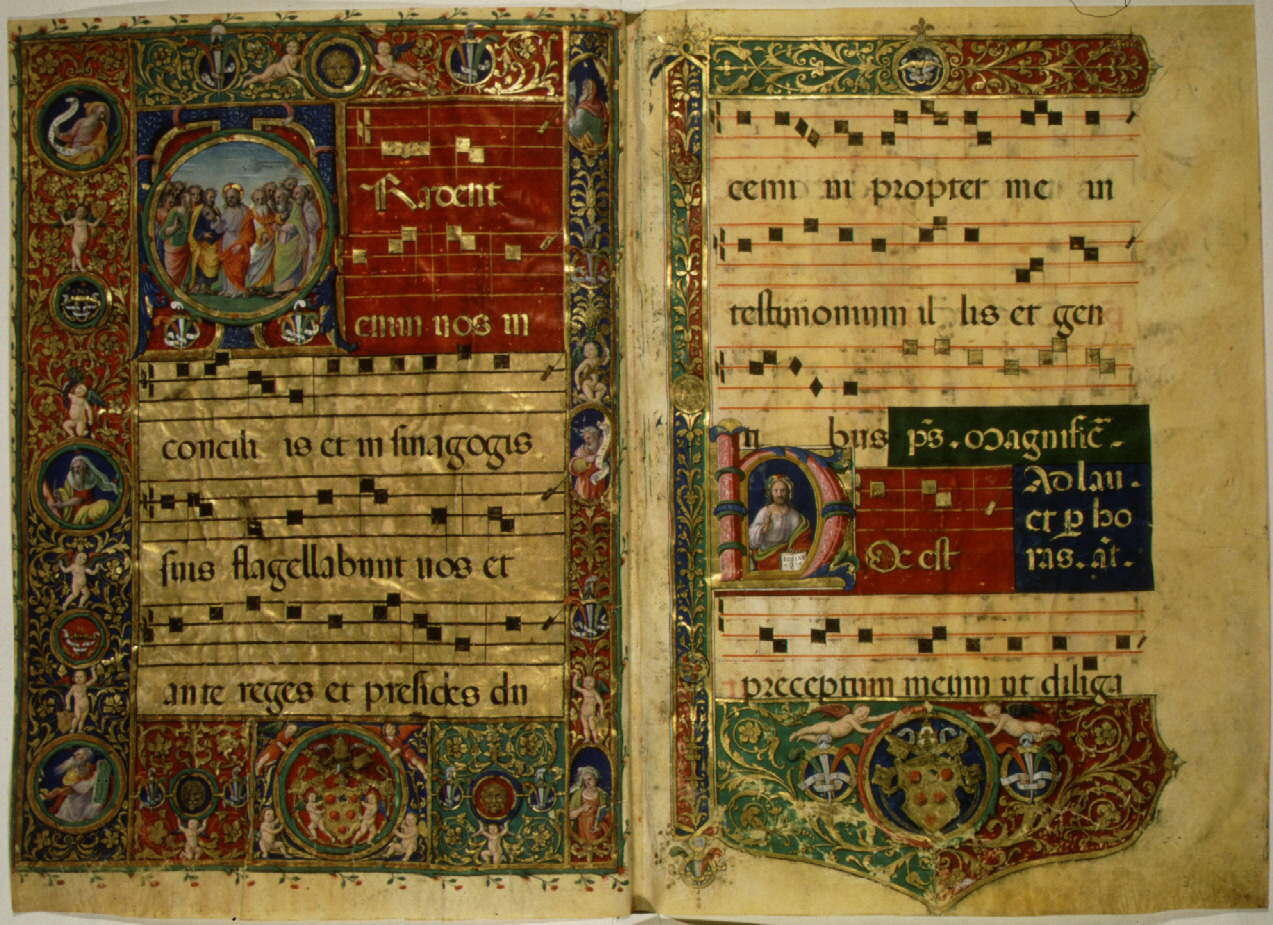
\includegraphics[width=.8\hsize]{chant.jpg}\hfil}
	
	%\medskip\pause
	%\uv{Spojování bodů} je přehledné, ale nemá matematický význam.
	%\pause
	%Nezbytně záleží na tom, \uv{kam se díváme}. \pause ($y = x^3 + 9x^2 - 10$)
	
\end{frame}


\begin{frame}
	\frametitle{Funkce daná předpisem}
	
	Například
	\[ f\colon y = \alt<-+>{\vphantom{\underbrace{x^3 + 9x^2 - 10}_{\text{funkční předpis}}}x^3 + 9x^2 - 10, \quad x \in \mathbb R}{\underbrace{x^3 + 9x^2 - 10}_{\text{funkční předpis}},\quad \underbrace{x \in \mathbb R}_{\rllap{$\scriptstyle\text{def. obor}$}}} \]
	%
	\pause
	Nebo stejně dobře tak
	\[ f(x) = x^3 + 9x^2 - 10,\quad \DO_f = \mathbb R \]
	\pause
	%
	Příklad s menším definičním oborem:
	\[ f(x) = \sqrt{x},\quad x \in \langle 0, \infty) \]
	
	\pause
	\begin{alertblock}{Pozor:}
	Definiční obor by \emph{měl být} součástí zadání funkce, ovšem typicky se bere jako definiční obor \alert{co největší množina reálných čísel}, pro kterou má funkční předpis smysl.
	\pause
	Odtud úlohy typu \uv{určete definiční obor funkce}.
	\end{alertblock}
	
	
\end{frame}


\section{Dodatek}


\begin{frame}
	\frametitle{$\star$ Děsivé funkce}
	\pause
	Ve skutečnosti se \uv{drtivá většina} reálných funkcí nedá zadat ani jedním z těchto způsobů.\pause
	
	Např.
	\begin{itemize}
		\item Cantorova funkce (\uv{Ďáblovo schodiště})
		
		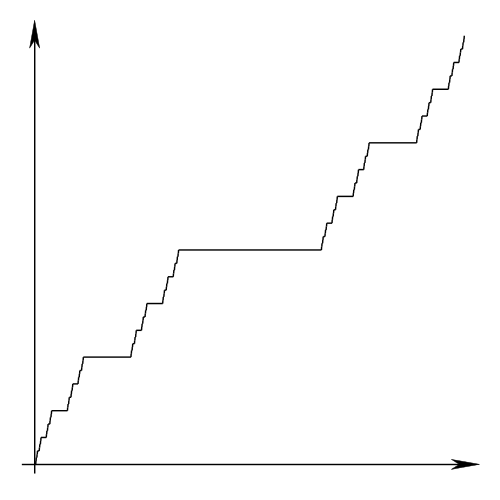
\includegraphics[width=.25\hsize]{cantor.png}
		\pause
	  \item Funkce, která mezi každými dvěma reálnými čísly nabývá všech reálných čísel
	\end{itemize}
\end{frame}


\end{document}
